\documentclass[11pt]{article}
\newcommand\tab[1][1cm]{\hspace*{#1}}
\newcommand\back[1][-3cm]{\hspace*{#1}}
\usepackage{graphicx}
\usepackage{soul}
\usepackage{amssymb}
\graphicspath{ {./lin/images} }
\begin{document}
\section{Lineare Gleichungssysteme und Gauss elimination}
Ein Gleichungssystem ist linear falls man kann ihn in diese Art schreiben:
\begin{equation}
	Ax+By=C
\end{equation}
Wo A und B darfen nicht gleichzeitig 0 sein.\\
Erst tauschen wir die Gleichungssystem in eine Matrix:
\begin{equation}
	A*x=b
\end{equation}
Wo A sind die Koeffizienten von die Gleichungen, x die Unbekanten und b die Lösungen.
Fur die Auflösung, tauschen wir die Matrix A in eine diagonalisierte matrix durch pivotierung.\\
In eine Gaus elimination darfen wir:
\begin{enumerate}
	\item Zeile vertauschen
	\item Addition und Subtraktion eines vielfachen der pivotzeile zu eine andere Zeile.
\end{enumerate}
Eine quadratische lineare Gleichungssystem wo eindeutige Lösungen berechenbar sind is \hl{regular}, sonst ist er \hl{singular}.
\paragraph{Rang}
Der rang eine Matrix ist die Anzahl von lineare unabhängige Zeilen (Anzahl pivotelemente).\\Die Anzahl der freien variablen ist n - r.\\
Der Gleichungssytem hat mindestens eine Losung wenn:
\begin{enumerate}
	\item $r = m$
	\item  $r < m$ und $c_{r+1} = c_{r+2} = c_m = 0$
\end{enumerate}
Gibt es losungen dann:
\begin{enumerate}
	\item $r = n \Rightarrow$ losung ist eindeutig.
	\item $r < n \Rightarrow$ gibt eine n - r parametrige losungsschar.
\end{enumerate}
\back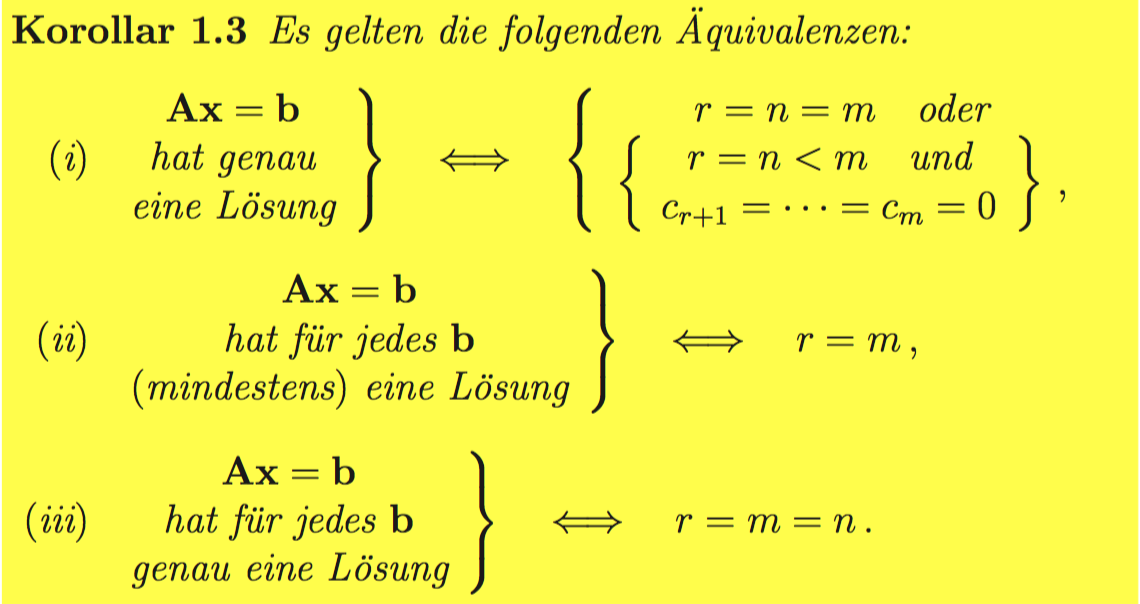
\includegraphics{images/gauss}\\
Ein Gleichungssytem heisst \hl{homogen} falls die rechte Seite aus nullen besteht.
\section{Matrizen und Vektoren}
\subsection{Notation}
$A_{xy}$ x ist die vertikale und y die Horizontale.\\
$\mathbb{R}^{m\times n}$ und $\mathbb{C}^{m\times n}$\\Sind die mengen reelen und complexen Matrizen.\\$\mathbb{E}^{m\times n}$ ist die Menge alle Matrizen.\\
\subsection{Rechnen mit Matrizen}
$A_{m\times n}\times B_{n\times p} = AB_{m\times p}$\\
\back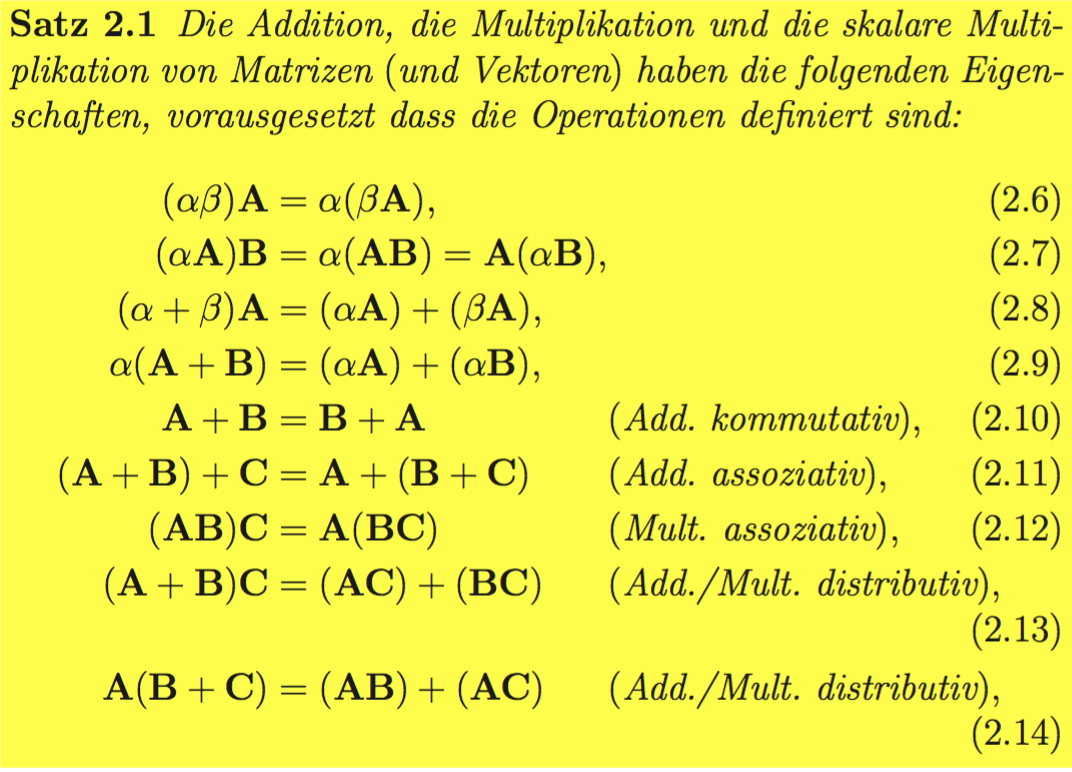
\includegraphics{images/matrizen}\\
$A\times B = O$ auch wenn $A\neq O \wedge B\neq O$\\
ist A eine m$\times$n Matrix, dann ist $A^T$die n$\times$m, die transponierte Matrix. Gleiche bei komplexe Zahlen mit die konjugiert-komplexe:$A^H$ von $\overline{A}$\\
Eine Matrix ist symmetrisch/hermitesch falls $A^H = A$ und ist schiefsymmetrisch falls $A^T = -A$\\$(AB)^T = B^TA^T$\\$A^TA und AA^T$ sind immer symmetrisch.
\subsection{Skalarprodukt, die norm, lange und Winkel von Vektoren}
\begin{equation}
	\parallel x\parallel = \sqrt{x_1^2+x_2^2+...+x_n^2}
\end{equation}
\paragraph{Der Cosinussatz:}
\begin{equation}
	\parallel y-x\parallel^2=\parallel x\parallel^2+\parallel y\parallel^2-2\parallel x\parallel\parallel y\parallel cos\varphi
\end{equation}
\paragraph{Skalarprodukt}
\begin{equation}
	\langle x,y\rangle := x_1y_1+x_2y_2
\end{equation}
\begin{equation}
	cos\varphi = \frac{\langle x,y\rangle}{\parallel x\parallel\parallel y\parallel}
\end{equation}
\back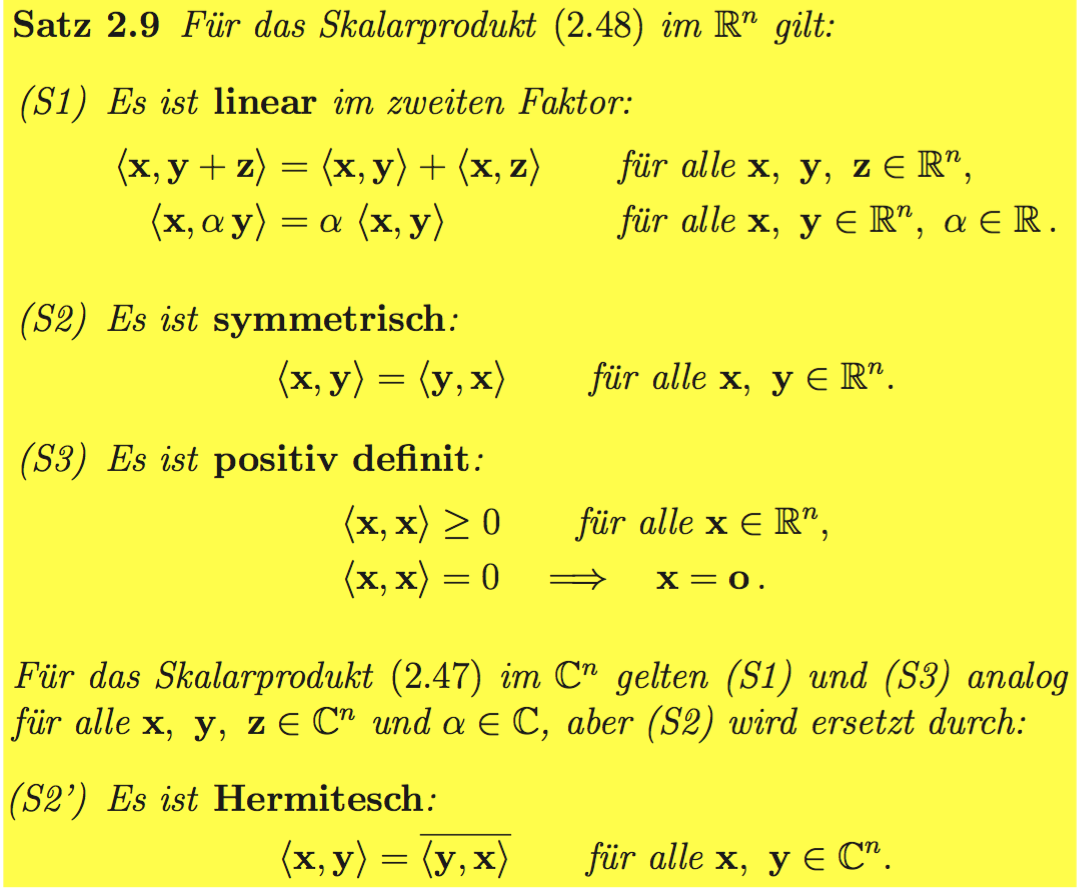
\includegraphics{images/skalarprodukt}\\
\back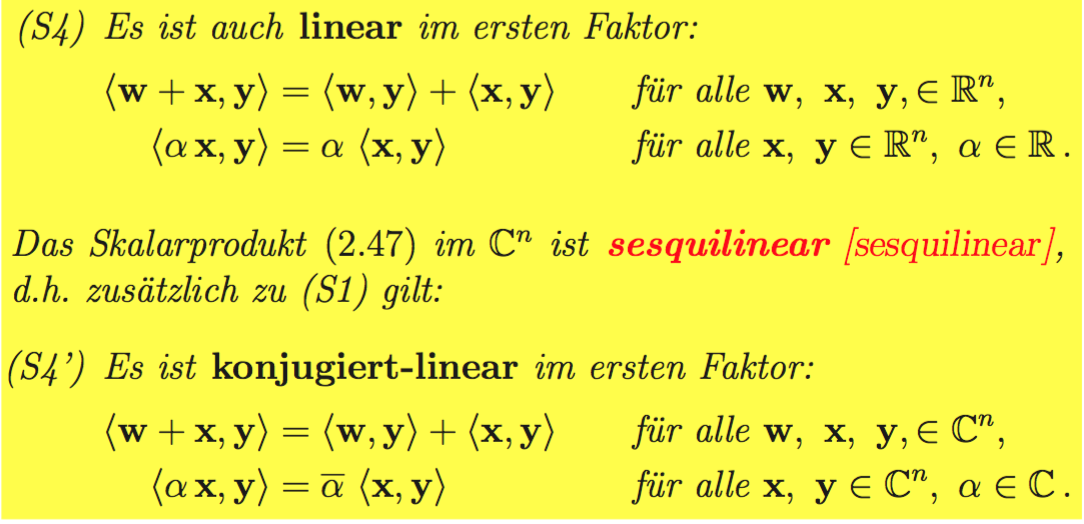
\includegraphics{images/skal}\\
\paragraph{Lange eine vektor:}
\begin{equation}
	\parallel x\parallel=\sqrt{\langle x,x\rangle}=\sqrt{x^Tx}
\end{equation}
\paragraph{Die schwarze ungleichung:}
\begin{equation}
	|\langle x,y\rangle|\le \parallel x\parallel \parallel y\parallel 
\end{equation}
\paragraph{Die norm}
\begin{enumerate}
	\item positiv definit: $\parallel x\parallel \ge 0, \parallel x\parallel =0 \Rightarrow x=0$
	\item Sie ist dem Betrage nach homogen: $\parallel \alpha x\parallel = |\alpha|\parallel x\parallel $
	\item Die Dreiecksungleichung: $\parallel x\pm y\parallel^2 \le \parallel x\parallel^2 +\parallel y\parallel^2$ fur alle x, y
\end{enumerate}
\begin{equation}
	\parallel x\parallel _p:=(|x_1|^p+...+|x_n|^P)^\frac{1}{p}
\end{equation}
\begin{equation}
	\parallel x\parallel _{\infty}:= max |x_k| k=1,...,n
\end{equation}
\paragraph{Senkrecht}
\begin{equation}
	\langle x,y\rangle=0 \Rightarrow x\perp y
\end{equation}
fals $x\perp y$ gillt:
\begin{equation}
	\parallel x\pm y\parallel^2=\parallel x\parallel^2+\parallel y\parallel^2
\end{equation}
\subsection{Das  ̈aussere Produkt und die orthogonale Projektion auf eine Gerade}
\subsubsection{Aussere Produkt}
Die aussere produkt eine m Vektors x une eines n vektors y ist die $m\times n$ Matrix $xy^H$\\Eine m$\times$n Matrix hat genau dann den Rang 1, wenn sie das  ̈aussere Produkt eines m–Vektors x$\neq$o und eines n– Vektors y$\neq$o ist.
\subsubsection{Orthogonale Porjektion}
Die orthogonale Projektion $P_yx$ des n–Vektors x auf die durch die Vielfachen von y ($\neq$o) erzeugte Gerade durch den Ursprung ist gegeben durch:
\begin{equation}
	P_yx := uu^Hx
\end{equation}
wo
\begin{equation}
	u := \frac{y}{\parallel y\parallel}
\end{equation}
\subsection{Matrizen als lineare Abbildungen}
\begin{equation}
	A: \mathbb{E}^n\rightarrow \mathbb{E}^m, x\mapsto Ax
\end{equation}
\paragraph{Der bild von A}
\begin{equation}
	im  A := \{Ax \epsilon \mathbb{E}^m; x \epsilon\mathbb{E}^n\}
\end{equation}
\subsection{Die inverse Matrix}
\begin{equation}
	AA^-1=I_n
\end{equation}
Die folgende aussangen sind equivalent:
\begin{enumerate}
	\item A ist invertierbar
	\item es gibt genau ein $A^-1$
	\item A ist regular, rang A = n
\end{enumerate}
\begin{equation}
	(AB)^-1 = b^-1A^-1
\end{equation}
\begin{equation}
	(A^T)^-1 = (A^-1)^T
\end{equation}
\subsection{Orthogonale und unit ̈are Matrizen}
Eine Matrix heisst unitar falls $A^hA = I_n$, heisst auch orthogonal falls $A^TA = I_n$\\
falls A und B sind unitare:
\begin{enumerate}
	\item $A^-1$ ist unitar
	\item AB ist unitar
\end{enumerate}
Eine unitare abbildung ist:
\begin{enumerate}
	\item length preserving
	\item angle preserving
\end{enumerate}
Therefore:
\begin{equation}
	\parallel Ax\parallel = \parallel x\parallel,	\langle Ax, Ay\rangle = \langle x,y\rangle
\end{equation}
\subsection{Strukturierte Matrizen}
Mehrere Type von Matrizen. schau im skript 2.9
\section{Die LR-Zerlegung}
\begin{equation}
	PA=LR
\end{equation}
Die Matrix A ist umgewandelt in eine obere und untere Dreieckmatrix.
\begin{equation}
	Lc=Pb
\end{equation}
\begin{equation}
	Rx=c
\end{equation}
Wir losen die zwei letzte durch Ruckwertseinsetzen und Vorwartseinsetzen.
\subsubsection{Die L matrix}
Die L matrix hat 1 auf die Diagonale und der Rest sind die inversen der Termen mit dem ich hab die Pivotzeilen multipliziert in der gauss algorithmus.
\subsubsection{Die R matrix}
Ist die obere Dreiecksmatrix die ich mit gauss erhalte.\\
wenn wir die lr zerlegung fur ein parameter machen und wir erhalten ein x uber dies parameter, dann hat a eine eindeutige losung fur jede parameter.
\subsection{Die LDR zerlegung}
\begin{equation}
	PA=LDR_1
\end{equation}
\begin{equation}
	R_1:=D^-1R
\end{equation}
D ist gleich die Pivotelemente.
\subsection{Untermatrizen fur LR zerlegung}
Eine m×n Matrix A vom Rang r l ̈asst sich genau dann ohne Zeilenvertauschungen LR–zerlegen, wenn die r fu ̈hrenden Hauptuntermatrizen $A_k$ (k=1,...,r)regul ̈ar sind.\\
\back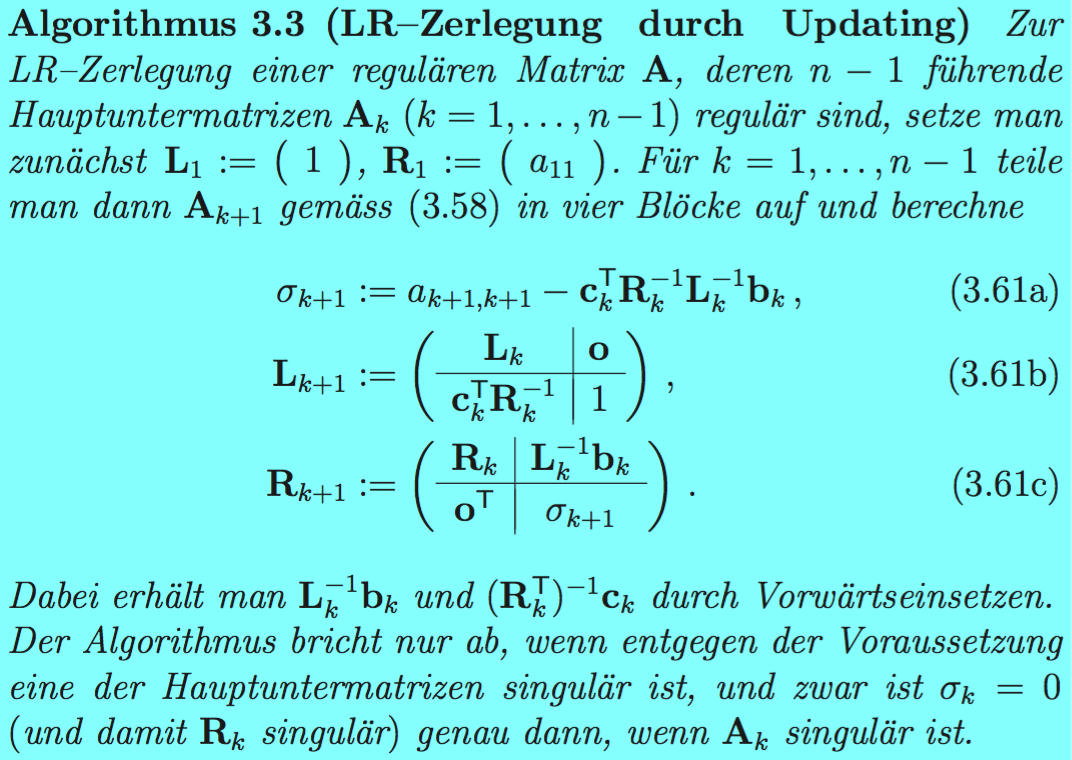
\includegraphics{images/updating}\\
\subsection{Die Cholesky-Zerlegung}
Wir nehmen die PA = LD$R_1$ zerlegung wo D ist die diagonale von R.\\Falls A symmetrisch ist dann ist P = I, und $R_1 = L^T$.
\begin{equation}
	A=LDL^T
\end{equation}
Jetzt kann mann setzen
\begin{equation}
	R_2 := D^\frac{1}{2}L^T
\end{equation}
\paragraph{Cholesky Zerlegung}
\begin{equation}
	A = R_2^TR_2
\end{equation}
\subsubsection{Positiv definit}
Eine reell symmetrische n × n Matrix A heisst positiv definit falls:
\begin{equation}
	x^TAX > 0 (\ge dann positiv semidefinit)
\end{equation}
Eine reell symmetrische oder Hermitesche Matrix, die positiv definit ist, ist regul ̈ar.
\section{Vektorr ̈aume}
Die Elemente einer bestimmten Menge lassen sich in natu ̈rlicher Weise addieren und mit einer reellen (oder komplexen) Zahl multiplizieren (“strecken”), wobei das Resultat beider Operationen je wieder ein Element der Menge ist und gewisse einfache Regeln gelten.\\Die axiome von Vektorraume:\\
\back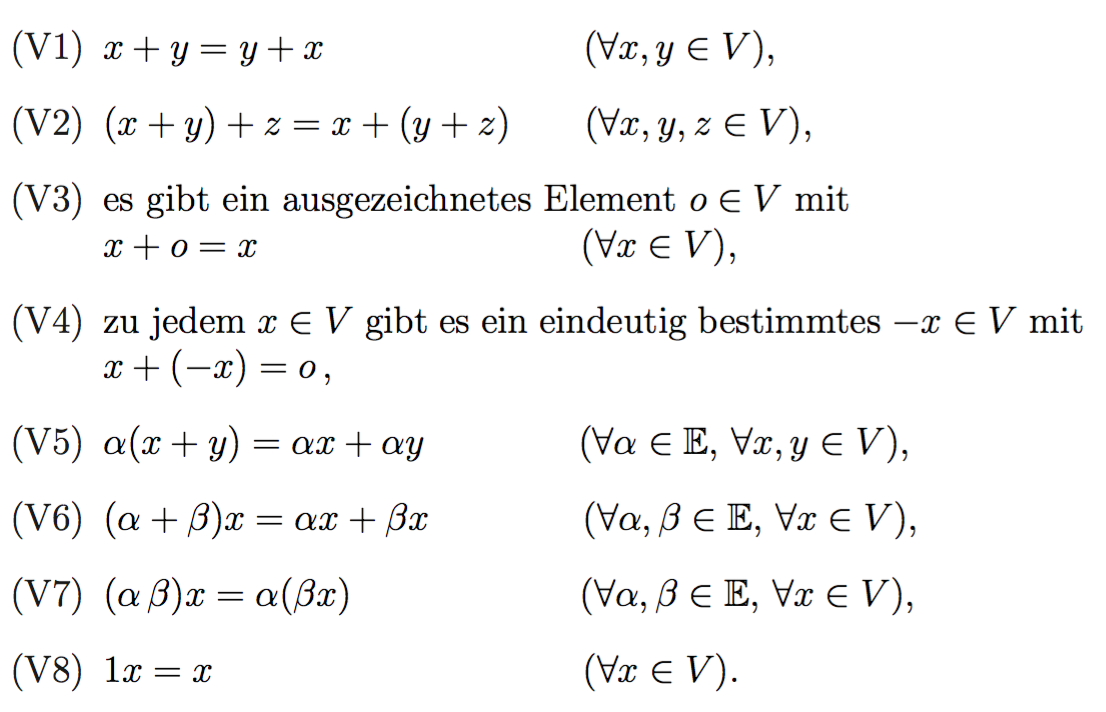
\includegraphics{images/verktorraum}\\
Es sei V ein Vektorraum u ̈ber $\mathbb{E}$. Fu ̈r alle x, y $\epsilon$ V und alle $\alpha \epsilon \mathbb{E}$ gilt:
\begin{equation}
	0x=o
\end{equation}
\begin{equation}
	\alpha 0=o
\end{equation}
\begin{equation}
	\alpha x = o \Rightarrow \alpha = 0 \vee x = o
\end{equation}
\begin{equation}
	(-\alpha)x=\alpha(-x)=-(\alpha x)
\end{equation}
Zu x,y $\epsilon$V existiert z $\epsilon$V mit x+z=y,wobei z eindeutig bestimmt ist und gilt: z = y + (−x).
\paragraph{Substraction:}
\begin{equation}
	y-x=y+(-x)
\end{equation}
\subsection{Korper}
Ein Ko ̈rper [field] ist eine nichtleere Menge K auf der eine Addition und eine multiplication definiert sind. Mit folgende Axiome:\\
\back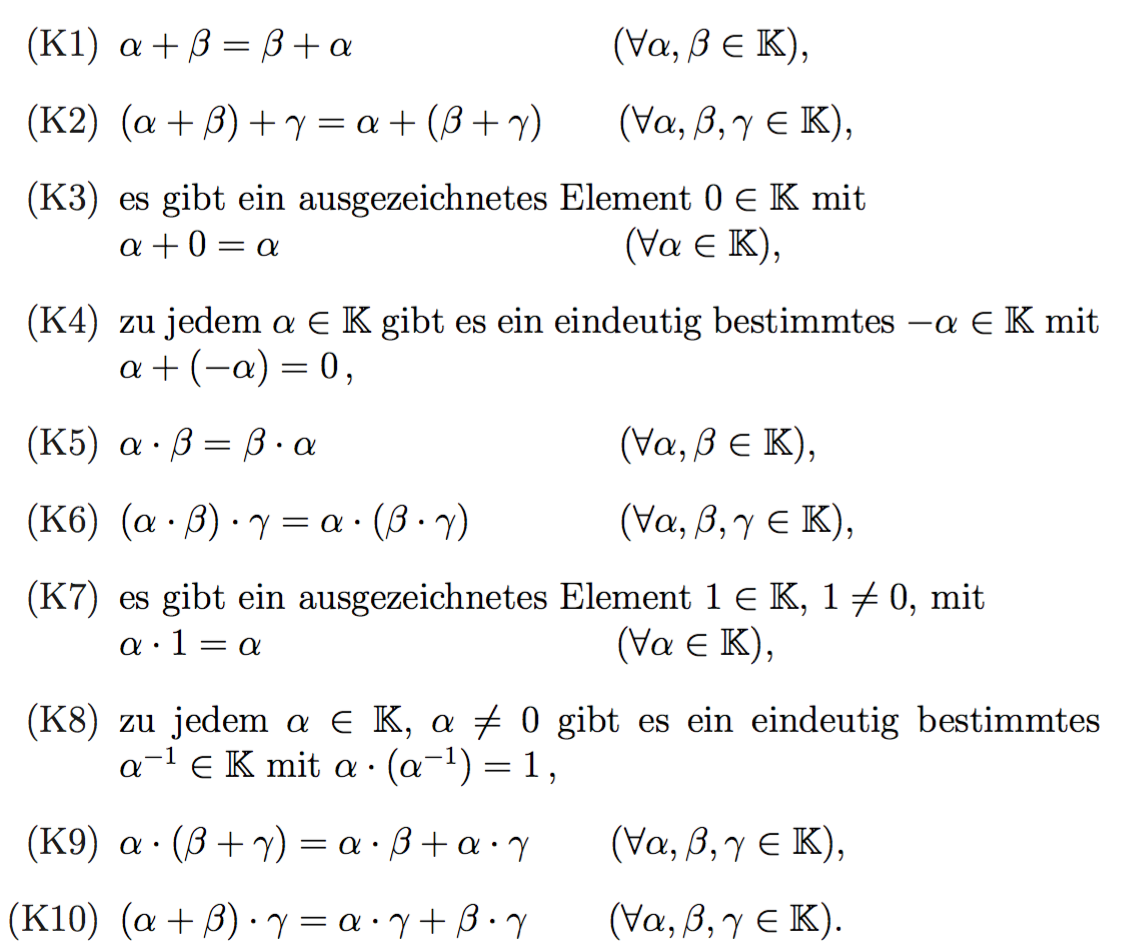
\includegraphics{images/feld}
\subsection{Unterr ̈aume, Erzeugendensysteme}
Eine nichtleere Teilmenge U eines Vektorraums V heisst Unterraum [subspace], falls sie bezu ̈glich Addition und ska- larer Multiplikation abgeschlossen ist.
\begin{equation}
	x+y \epsilon \mathbb{U},\alpha x \epsilon \mathbb{U} (\forall x,y \epsilon \mathbb{U}, \forall \alpha \epsilon \mathbb{E})
\end{equation}
Ein Unterraum ist selbst ein Vektorraum.
\subsubsection{Lineare Hulle}
Die Menge aller Linearkombinationen von a1, . . . , al heisst der von a1, . . . , al aufgespannte (oder: erzeugte) Un- terraum [subspace spanned by a1,...,al; span] oder die lineare Hu ̈lle von a1, . . . , al [linear hull]:\\
\tab span \{$a_1,..,a_l$\} := \{$\sum y_ka_k; y_1,..,y_l \epsilon \mathbb{E}$\}\\
die vetoren $a_1,..a_l$ sind Erzeugendensystem [die spanning set] von span.
\subsection{Basen}
Ein linear unabha ̈ngiges Erzeugendensystem eines Vektorraums V heisst Basis [basis] von V.\\
Besitzt ein Vektorraum V ein endliches Erzeugendensy- stem, so besteht jede Basis von V aus derselben Zahl von Vektoren.
\paragraph{Dimension}
Die Zahl der Basisvektoren (in jeder Basis) eines Vektorraumes V mit endlichem Erzeugensystem heisst Dimensi- on [dimension] von V und wird mit dim V bezeichnet.\\
Zwei Unterra ̈ume U und U′ eines Vektorraumes V mit der Eigenschaft, dass jedes x $\epsilon$ V eine eindeutige Darstellung hat, heissen komplement ̈ar [complementary]. Wir nennen dann V die direkte Summe [direct sum] von U und U′ und schreiben:
\begin{equation}
	V = U \oplus U'
\end{equation}
\subsection{Basiswechsel, Koordinatentransformation}
Wir konnen die koordinaten von ein Punkt in eine Basis in die Koordinate von ein neue Basis umwalden indem wir eine Basiswechselmatrix benutzten. Die invers von diese Matrix macht der umgekehrte weg.
\section{Lineare Abbildungen}
Eine Abbildung zwischen zwei Vektorra ̈umen heisst linear, wenn sie “die linearen Beziehungen invariant (un- vera ̈ndert) la ̈sst”. Wa ̈hlt man in den Vektorra ̈umen Basen, so in- duziert eine solche Abbildung eine lineare Abbildung der Koordi- naten. Falls die Ra ̈ume endlich-dimensional sind, wird diese durch eine Matrix repra ̈sentiert. Dies ist, in Ku ̈rze, der grundlegende Zu- sammenhang zwischen linearen Abbildungen und Matrizen.
\subsection{Definition, Beispiele, Matrixdarstellung}
Ist F bijektiv, so ist die inverse Abbildung [inverse map, inverse mapping, inverse transformation] F−1 definiert.\\
F ist surjektiv falls rang F = dim von abbildungs Matrix, F ist injektiv falls die spaltenvektoren unabhangig sind.
\back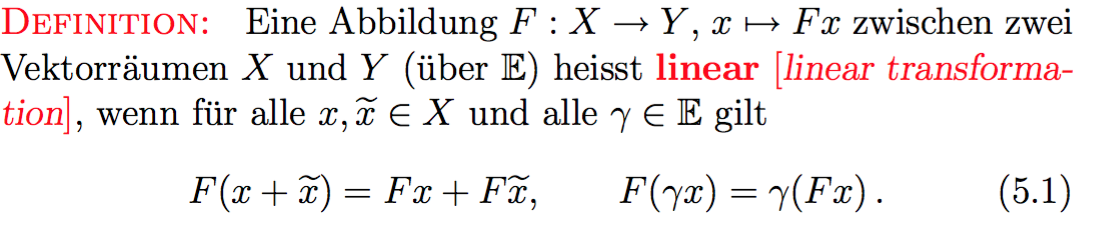
\includegraphics{images/linear}\\
X ist der Definitionsraum [domain], Y der Bildraum [image space] der Abbildung.
\paragraph{Isomorphismus}
Eine eineindeutige lineare Abbildung von X auf Y heisst Isomorphismus [isomorphism]. Ist X = Y , so heisst sie Automorphismus [automorphism].\\
st F : X $\rightarrow$ Y ein Isomorphismus, so ist die inverse Abbildung $F^-1$ : Y $\rightarrow$ X linear und auch ein Isomorphismus.
\paragraph{kommutative Diagramm:}
\back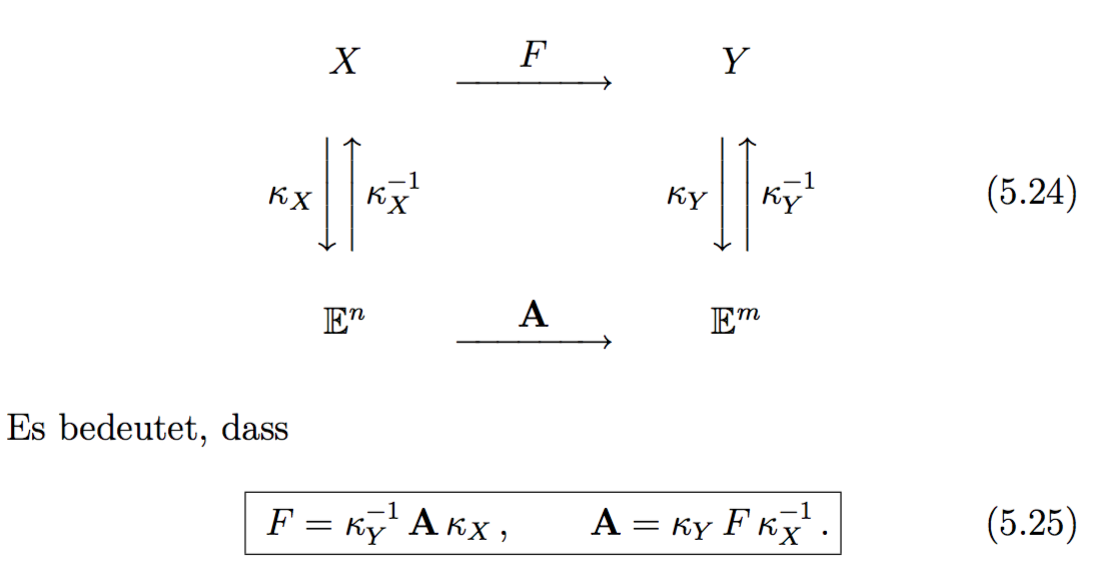
\includegraphics{images/diagram}
\subsection{Kern, Bild und Rang}
\begin{equation}
	F:X\rightarrow Y
\end{equation}
Wo dim X = n, dim Y = m.
\subsubsection{Kern}
Der Kern [kernel] ker F von F ist das Urbild von o $\epsilon$ Y.
\begin{equation}
	ker f := \{x \epsilon X; Fx = o \} \subseteq X
\end{equation}
Ker f is ein Unterraum von X, und im F ist ein Unterraum von Y.\\
Ist U ein Unterraum von X, so ist dessen Bild FU ein Unterraum von Y. Ist W ein Unterraum von im F, so ist dessen Urbild F°1W ein Unterraum von X.\\
F ist genau dann injektiv, wenn ker F = \{o\} ist.
\begin{equation}
	dimX - dim ker F = dim im F
\end{equation}
Um eine Base von kern zu finden: losen wir einfach die Matrix Ax = 0;\\
Um eine base von bild zu finden: Wir konnen einfach nehmen die spalten die linear unabhangig sind (die die Pivotelemente haben).
\subsubsection{Rang}
Der Rang [rank] einer linearen Abbildung F ist gleich der Dimension des Bildes von F.\\
\back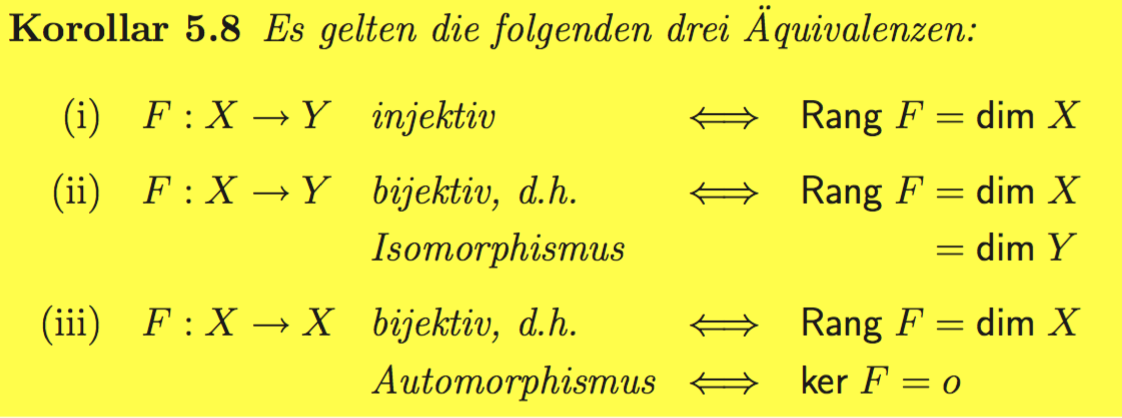
\includegraphics{images/rang}
\subsubsection{Isomorph}
Zwei Vektorra ̈ume X and Y heissen isomorph, falls es einen Isomorphismus F : X $\rightarrow$ Y gibt.\\
Zwei Vektorr ̈aume endlicher Dimension sind genau dann isomorph, wenn sie die gleiche Dimension haben.\\
\back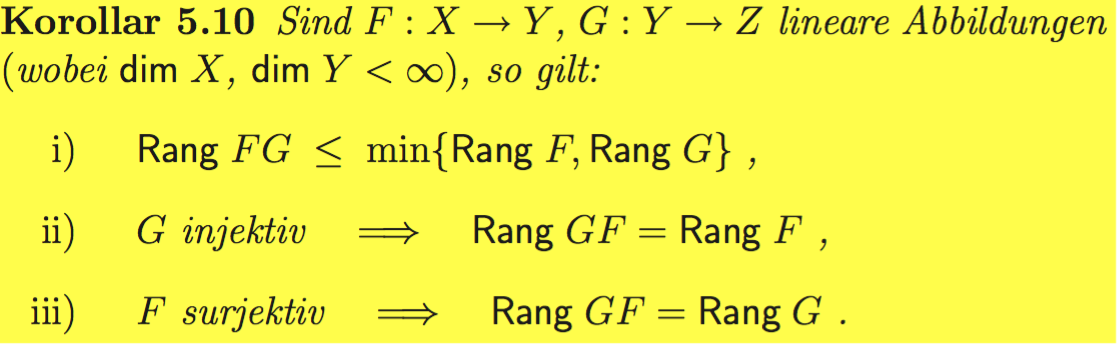
\includegraphics{images/iso}\\
\subsection{Matrizen als lineare Abbildungen}
$\Re (A)$ :+ span\{$a_1,...,a_n$\} wo a sind die kollonenvektoren von A. $\Re (A)$ ist der kolonnenraum von A = Im a.\\
Der losungsraum des homogenen systems Ax=o, heisst Nullraum $\aleph (A)$ = ker A.\\
Das Gleichungssystem Ax = b ist genau dann l ̈osbar, wenn b im Kolonnenraum von A liegt.\\
\back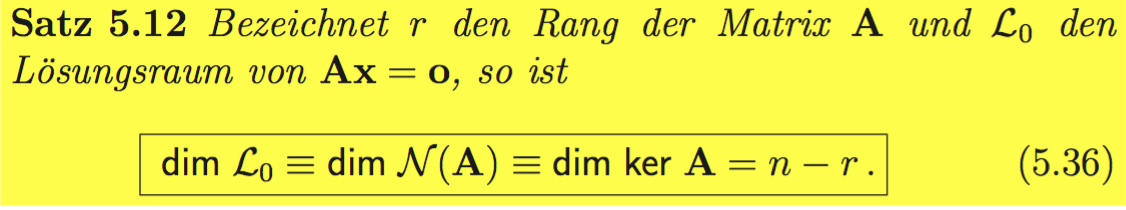
\includegraphics{images/mat}\\
Der rang einer m $\times$ n matrix A ist gleich:
\begin{enumerate}
	\item Anzahl Pivotelemente
	\item dim im A
	\item Dimensions des kolonnenraums (anzahl linear unabhangiger kolonnen).
	\item Dimesnions des Zeilenraums (anzahl linear unabhangiger Zeilen).
\end{enumerate}
$\Re (A)$ is gleich der Menge b fur die Ax=b eine losung x hat.\\
$A \epsilon \mathbb{E}^{m \times n}$, $B \epsilon \mathbb{E}^{p \times m}$ dann gilt:
\begin{enumerate}
	\item Rang BA $\leq$ min \{rang B, Rang A\}
	\item rang B = m$(\leq p)$ $\Rightarrow$ rang BA = rang A
	\item rang a = m$(\leq n)$ $\Rightarrow$ rang BA = rang B
\end{enumerate} 
$A \epsilon \mathbb{E}^{m \times m}$, $B \epsilon \mathbb{E}^{m \times m}$ dann gilt:
\begin{enumerate}
	\item Rang BA $\leq$ min \{rang B, Rang A\}
	\item rang B = m $\Rightarrow$ rang BA = rang A
	\item rang a = m $\Rightarrow$ rang BA = rang B
\end{enumerate} 
Matrix A $\epsilon \mathbb{E}^{n \times n}$ sind folgende aussagen aquivalent:
\begin{enumerate}
	\item A ist invertiebar
	\item A ist regular
	\item Rang A = n
	\item kollonenvektoren und Zeilenvektoren sind linear unabhangig
	\item im A := $\Re (A) = \mathbb{E}^n$
	\item ker A := $\aleph (A)$ = \{o\}
	\item die lineare Abbildung A : $\mathbb{E}^n \rightarrow \mathbb{E}^n$ ist ein Automorphismus
	\item A ist die Transformationsmatrix einer Koordinatentransformation in $\mathbb{E}^n$
	\item es gib kein k $k \epsilon \mathbb{N}$ sodass $A^k$ = 0.
	\item 
\end{enumerate}
Wenn die Matrix regular ist, dann Ax=0 hat keine nicht triviale losungen.
\subsection{Affine Raume und die allgemeine Losung eines inhomogenen Gleichungssystems}
Eine affiner teilraum, ist wenn wir zu einer Unterraum von V U ein teil von V addieren.\\
Eine affine Abbildung ist wenn wir zu eine Bildmenge von eine lineare Abbildung ein Teil von diese Menge addieren:$H : X \rightarrow y_0 + Y $,  $x \mapsto y_0 + Fx$\\
Die losungsmenge $\ell_b$ des affinen Teilraum Ax=b, ist gleich $\ell_0$ den losungsraum des homogenen systems Ax=o plus irgend eine losung des inhomogenen system $x_0$.
\begin{equation}
	\ell_b = \ell_0 + x_0
\end{equation}
\subsection{Die Abbildungsmatrix bei Koordinaten- transformation}
\back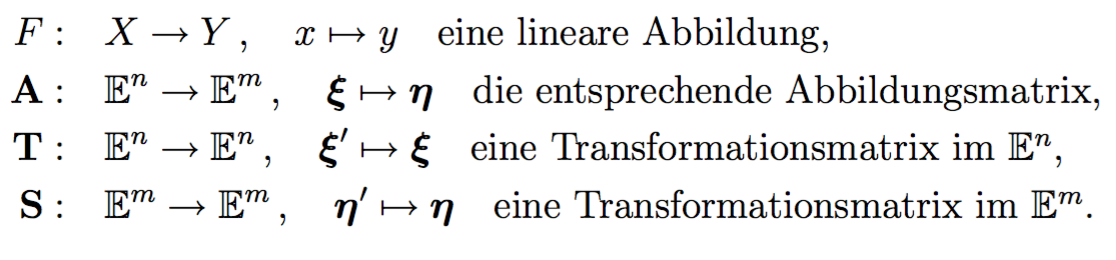
\includegraphics{images/1}\\
\back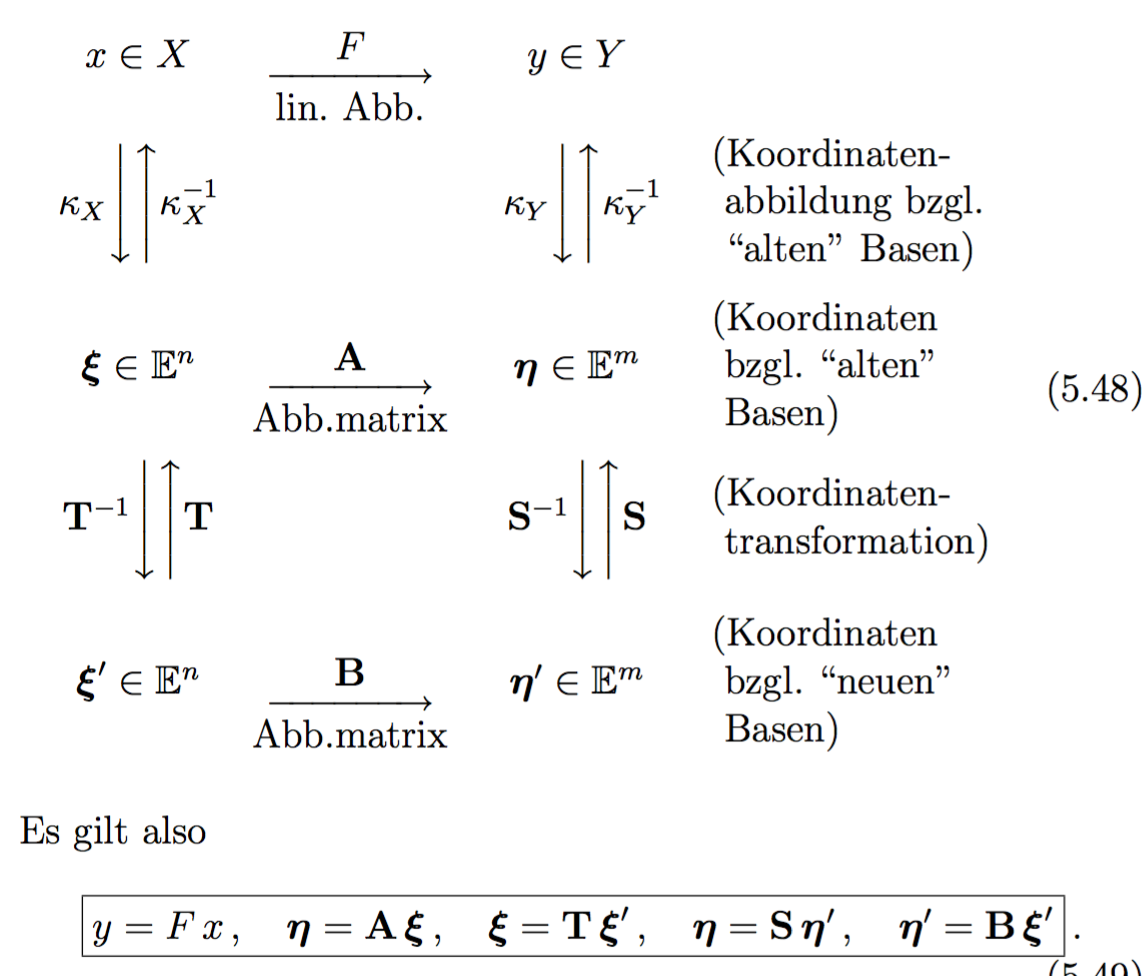
\includegraphics{images/2}\\
\paragraph{Anhlich}
A und B heissen ahnlich falls es existiert ein T sodass: $A \mapsto B = T^-1AT$
\section{Vektorr ̈aume mit Skalarprodukt}
\subsection{Norm}
Ein norm in ein Vektorraum:
\begin{equation}
	\parallel.\parallel: V \rightarrow\mathbb{R}, x \mapsto\parallel x\parallel
\end{equation}
Sie ist positiv definit, homogen und der Dreiecksungleichung gilt.\\
Ein Vektorraum mit einer Norm heisst normierter Vektorraum
\subsection{Vektorr ̈aume mit Skalarprodukt}
Skalarproduct in einem reelen oder komplexen Vektorraum:
\begin{equation}
	\langle.,.\rangle:V\times V \rightarrow \mathbb{E}, x,y \mapsto \langle x, y \rangle
\end{equation}
Er ist linear, symmetrisch und positiv definit(wie bei normalen skalarprodukt)\\
falls $\mathbb{E} = \mathbb{R}$ Euklidischer Vektorraum oder orthogonaler Vektorraum, falls$\mathbb{E} = \mathbb{C}$ unit ̈arer Vektorraum.
\paragraph{Schwarzsche ungleichung}
\begin{equation}
	\mid\langle x, y \rangle\mid \leq \parallel x \parallel \parallel y \parallel 
\end{equation}
Das Gleichheitszeichen gilt genau dann, wenn x und y linear
abh ̈angig sind.\\
Winkel ist gleich bei normal, und falls orthogonal dann skalarprodukt = 0.
\paragraph{Pythagores}
\begin{equation}
	x\perp \Rightarrow \parallel x\pm y \parallel^2 = \parallel x\parallel^2 + \parallel y \parallel^2
\end{equation}
\back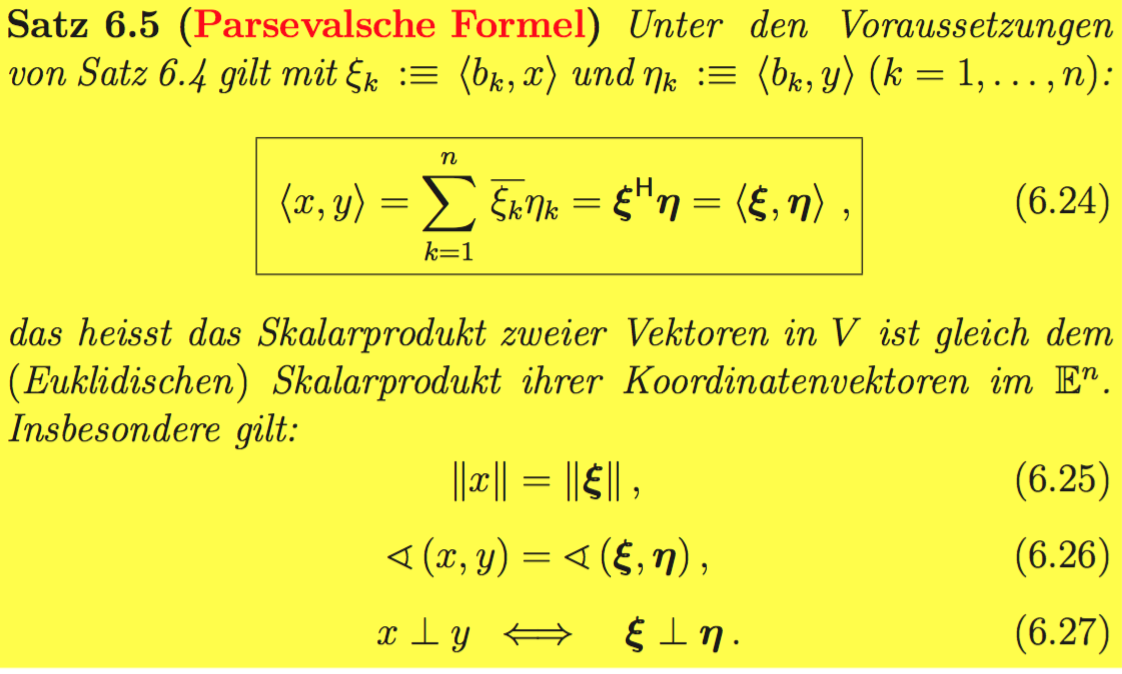
\includegraphics{images/parsevelsche}\\
\subsection{Gram schmidt algorithmus}
Um eine nicht orthogonale und nicht unitare Basis\{a1,...,an\} ein eine orthonormale basis\{b1,...,bn\} umwalden.
\begin{equation}
	b_1 := \frac{a_1}{\parallel a_1 \parallel}
\end{equation}
\begin{equation}
	b_{k'} := a_k-\sum_{j=1}^{k-1}\langle b_j,a_k\rangle b_j,
\end{equation}
\begin{equation}
	b_k := \frac{b_{k'}}{\parallel b_{k'}\parallel}
\end{equation}
Es gibt verschiedene Type von Vektorraume:
\begin{enumerate}
	\item topologischer Vektorraum(mit Umgebungsbegriff)
	\item Banachraum(mit Vektornorm)
	\item Hilbertraum(mit Skalarprodukt und zu-
geho ̈riger Vektornorm)
\end{enumerate}
\subsection{Orthogonale Komplemente}
In einem Vektorraum endlicher Dimension mit Skalarprodukt kann man jede Menge orthonormaler Vektoren zu einer orthonormalen Basis erg ̈anzen.
\paragraph{orthogonale komplement}
In einem endlich-dimensionalen Vektorraums V mit Skalarprodukt heisst der zu einem echten Unterraum U orthogo- nale komplementa ̈re Unterraum das orthogonale Komplement von U und wird mit $U^{\perp}$
\begin{equation}
	U^{\perp} := \{x\epsilon V; x \perp U\}
\end{equation}
Wir nennen dann V eine direkte Summe orthogonaler Komplemente
\begin{equation}
	dim U + dim U^{\perp} = dim V
\end{equation}
\back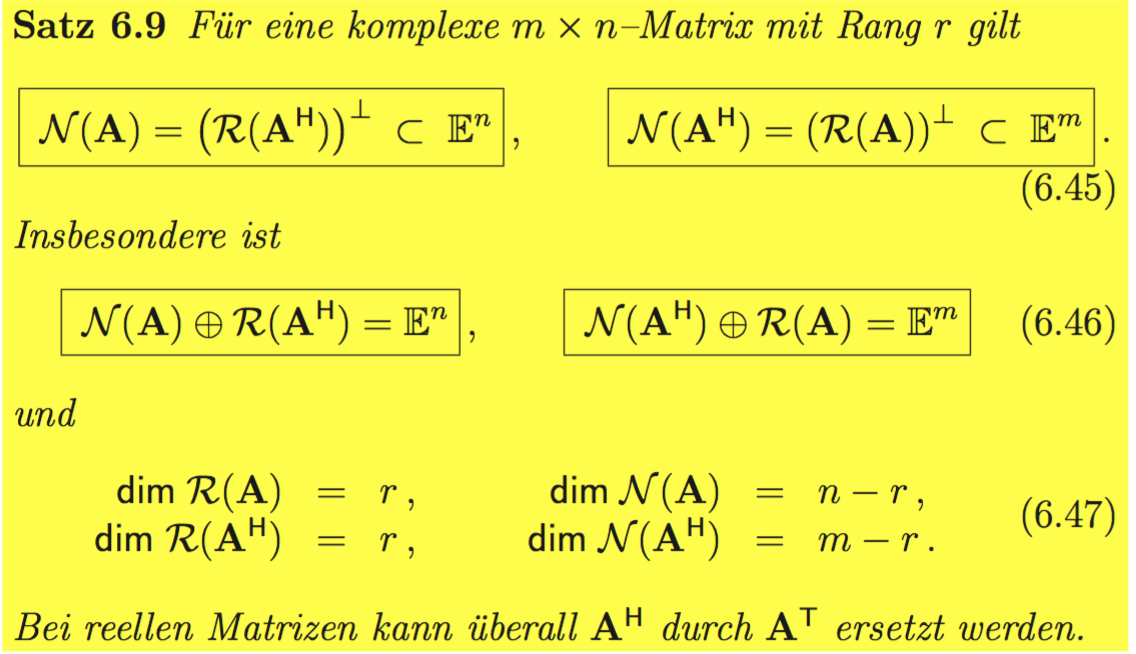
\includegraphics{images/komplexe}
\subsection{Orthogonale und unit ̈are Basiswechsel und Koordinatentransformationen}
Wenn beide Basen sind orthonormal dann:
\begin{equation}
	I=T^TT
\end{equation}
Die invers von der basiswechselmatrix $T^-1=T^T$ vereinfachet viel die Rechnung\\
\back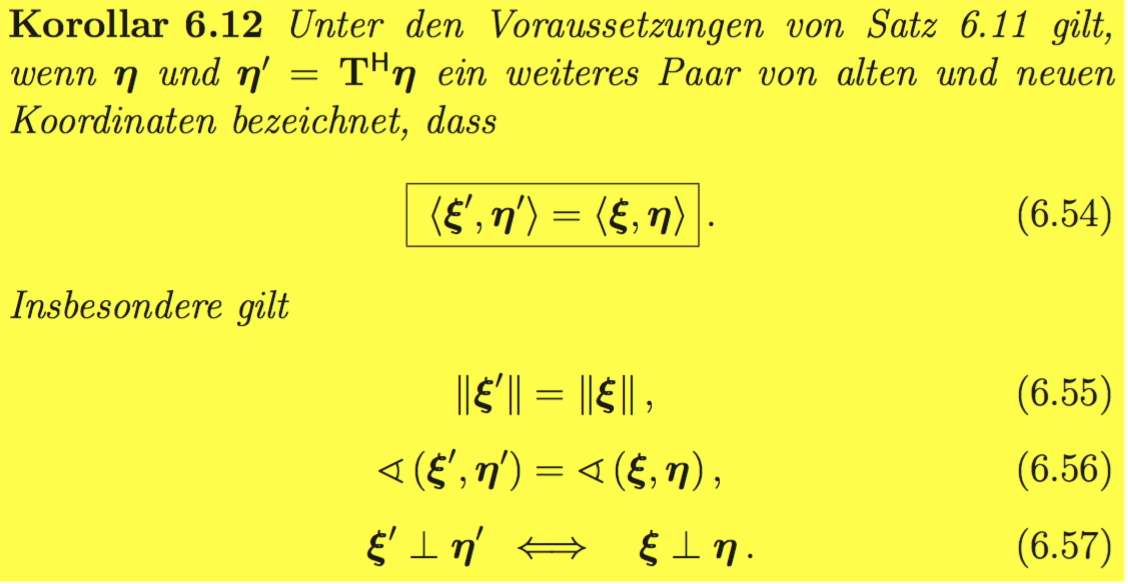
\includegraphics{images/wechsel}
\subsection{Orthogonale und unit ̈are Abbildungen}
Ein Abbildung F heisst unitar falls er zwischen zwei untare Vektorraume ist und:
\begin{equation}
	\langle Fx, Fy\rangle_Y = \langle x,y \rangle_X
\end{equation}
\back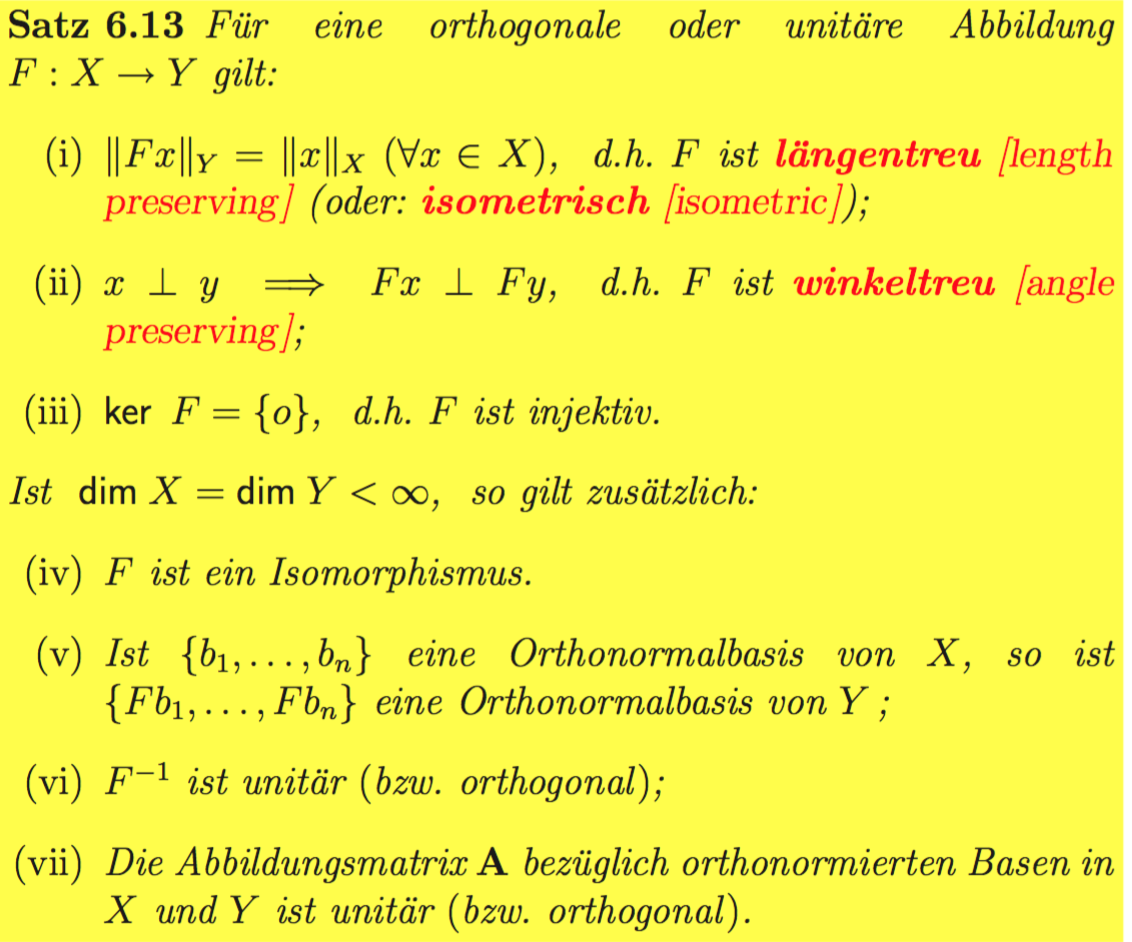
\includegraphics{images/unitar}\\
Wenn F und G sind unitar dann ist auch FoG unitar\\
Eine Matrix ist unitar wenn seine abbildung unitar ist
\subsection{Normen von linearen Abbildungen (Operatoren) und Matrizen}
Eine lineare Abbildung heisst beschrankt wenn es ein $\gamma$ exisitier sodass:
\begin{equation}
	\parallel F(x)\parallel_Y \leq \gamma\parallel x\parallel_X, (\forall x \epsilon X)
\end{equation}
Die Gesamtheit solcher linearer Abbildungen (Operatoren) F zwischen X und Y heisst $\ell (X,Y)$\\
Die operator Norm hat die folgenden Eigenschaften:
\begin{enumerate}
	\item positiv definit
	\item homogen
	\item dreicksungleichung
	\item $\parallel F\circ G\parallel \leq \parallel F\parallel + \parallel G \parallel$
	\item $\parallel Fx\parallel_Y \leq \parallel F\parallel \parallel x\parallel_X$,  $(\forall F \epsilon \ell(X,Y), \forall x \epsilon X)$  
\end{enumerate}
\paragraph{Matrix norm}
Ist eine Norm die hat alle diese Eigenschaften
\paragraph{Konditionszahl}
\begin{equation}
	\kappa(A) = \parallel A\parallel \parallel A^-1\parallel
\end{equation}
\section{Die Methode der kleinsten Quadrate und die QR–Zerlegung einer Matrix}
\subsection{Orthogonalprojektionen}
Eine lineare Abbildung $P: \mathbb{E}^m \rightarrow \mathbb{E}^m$ heisst Projektion falls:
\begin{equation}
	P^2=P
\end{equation}
Eine Projektion heisst Orthogonalprojektion falls:
\begin{equation}
	ker P \perp im P \Rightarrow N(P) \perp \Re (P)
\end{equation}
Sonst ist es eine schife projektion\\
Ist P ein projektor so ist auch I - P eine Projektor und im(I-P) = ker P, ker(I-P) = im P.\\
Fur ein Projektor:
\begin{enumerate}
	\item P is orthogonaler projektor
	\item I-P is orthogonaler projektor
	\item $P^T=P$
\end{enumerate}
Die Orthogonalprojektion PA den Kolonnenraum im A
\begin{equation}
	P_A := A(A^HA)^-1A^H
\end{equation}
Fu ̈r eine Orthogonalprojektion P gilt:
\begin{equation}
	\parallel y-Py\parallel_2 = min_{z\epsilon im P} \parallel y-z\parallel_2
\end{equation}
\subsection{Die Methode der kleinsten Quadrate}
Es gibt eine lineare Gleichungsystem Ax=y fur den weiss man, dass es kein losung gibt. Wir suchen also ein losung r := y - Ax sodass euklidische norm $\parallel r \parallel^2$ minimal wird.\\
Losung:
\begin{equation}
	A^TAx=A^Ty
\end{equation}
Wo x ist die losung.
\subsection{Die QR–Zerlegung einer Matrix}
Wir zerlegen die Matrix $m\times n$ A in QR, wo $m\times n$ Q ist eine orthonormalen Matrix und $n\times n$ rechtdreiecksmatrix R.\\
Wir finden Q mit der gramschmidt algorithmus und R:
\begin{equation}
	r_{kk} := \parallel q_{k'}
	r_{jk} := \langle q_j,a_k \rangle
\end{equation}
Mit der QR zerlegung konnen wir auch der kleinste quadrat finden mit:
\begin{equation}
	Rx = Q^Hy
\end{equation}
\subsection{Die QR–Zerlegung mit Pivotieren}
Wenn man die matrix zeilen tauschen will weil es irgendwo ein null gibt:\\
\back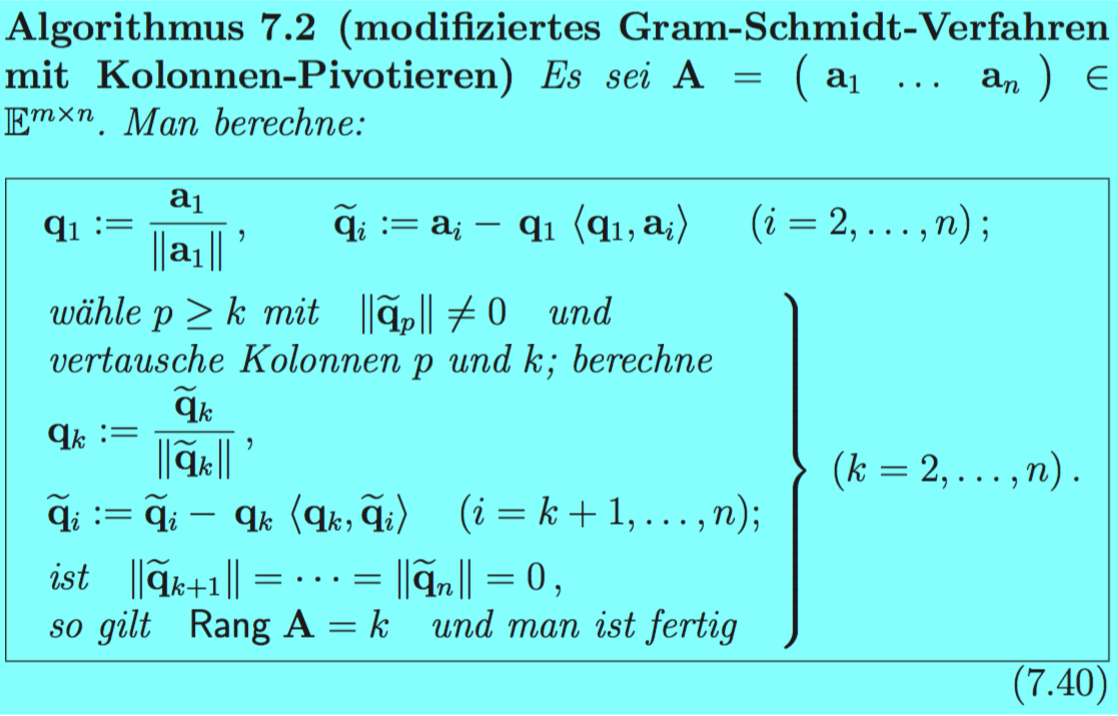
\includegraphics{images/gram}\\
\begin{equation}
	AP=QR
\end{equation}
\section{Determinaten}
\subsection{Permutationen}
Jede Permutation p als Produkt von Transpositionen tk benachbarter Elemente dargestellt werden, es kann mehrere oder wenige transpositonen geben aber sind immer gerade oder ungerade.\\
Det hat folgende eigenschaften:
\begin{enumerate}
	\item Hat a eine zeile aus nullen, so ist det A = 0
	\item det(yA) = $y^n$ det A
	\item Hat A zwei gleiche Zeilen, so ist det A = 0.
	\item Addiert man zu einer Zeile von A ein Vielfaches einer anderen Zeile von A, so  ̈andert sich der Wert von det A nicht.
	\item Ist A eine Diagonalmatrix, so ist det A gleich dem Produkt der Diagonalelemente.
	\item Ist A eine Dreiecksmatrix, so ist det A gleich dem Produkt der Diagonalelemente.
\end{enumerate}
\begin{equation}
	det A \neq 0 \iff rang a = n \iff A regular
\end{equation}
Durch Eigenschaft 4 kann mann der Determinante mit gauss finden.
\begin{equation}
	det(AB)= det A\cdot det B
\end{equation}
\begin{equation}
	det A^-1= (det A)^-1
\end{equation}
\begin{equation}
	det A^T = det A
\end{equation}
\subsection{Entwicklung nach Zeilen und Kolonnen}
Zu jedem Element akl einer n £ n–Matrix A werde die (n - 1) $\times$ (n - 1)–Untermatrix A[k,l] definiert durch Streichen der Zeile k und der Kolonne l von A.
\begin{equation}
	(-1)^{k+l}det A_{[k,l]}
\end{equation}
Wir wahlen eine zeile aus, dann gehen wir durch die Matrize auf diese zeile und addieren wir alle determinate von oben mal der erste zahl von diese zeile.
\section{Eigenwerte und Eigenvektoren}
\subsection{Eigenwerte und Eigenvektoren von Matrizen und linearen Abbildungen}
Die Menge aller Eigenwerte von F heisst Spektrum $\sigma(F)$\\
Die geometrische Vielfachheit eines Eigenwertes y ist gleich der Dimension von $E_y$
\begin{equation}
	dim E_y= dim ker(A-yI)
\end{equation}
Um die Eigenwerte zu finde : det(A - yI) = 0. Wir finden die y. Dann nehmen wir dies y und setzen wir in A - yI und die Vektoren fur die geht (A - yI)x=0 sind die Eigenvektoren.
\paragraph{Singular}
Eine (quadratische) Matrix A ist genau dann singul ̈ar, wenn sie 0 als Eigenwert hat.
\subsection{A ̈hnlichkeitstransformationen; die Eigenwertzerlegung}
 ̈Ahnlichen Matrizen haben dasselbe charakteristische Polynom; sie haben also die gleiche Determinante, die gleiche Spur und die gleichen Eigenwerte (A und B sind ahnlich wenn B = $T^-1AT$).
Eine zu F geh ̈orende Abbildungsmatrix ist genau dann diagonal, wenn die gew ̈ahlte Basis von V aus lauter Eigenvektoren von F besteht.\\
Eine Basis aus Eigenvektoren von F heisst Eigenbasis von F\\
A ist die Matrix V ist die eigenbasis und $\wedge$ ist die diagonal matrix:
\begin{equation}
	A = V \wedge V^-1
\end{equation}
wo $\wedge$ hat die eingenwerte auf die diagonale.\\
 Eigenvektoren zu verschiedenen Eigenwerten sind linear unabh ̈angig.\\
 Fu ̈r jeden Eigenwert gilt, dass die geometrische Viel- fachheit kleiner gleich der algebraischen Vielfachheit ist.\\
 Eine Matrix ist genau dann diagonalisierbar, wenn fu ̈r jeden Eigenwert die geometrische gleich der algebraischen Viel- fachheit ist.
\subsection{Eigenwerte und Eigenvektoren symmetrischer und Hermitescher Matrizen}
Fur symmetrischer Matrizen:
\begin{enumerate}
	\item alle eigenwerte sind reel
	\item Die reellen Eigenvektoren zu verschiedenen Eigenwerten sind paarweise orthogonal
	\item Es gibt eine orthonormale Basis aus Eigenvektoren u1,...,un von A.
	\item Fu ̈r die orthogonale Matrix U gilt :$U^TAU= \wedge:= diag(y_1,...,y_n)$
\end{enumerate}
\section{Singular wert Zerlegung}
Wir zerlegen A:
\begin{equation}
	A = U\Sigma V^T
\end{equation}
U und V sind orthonoramle unitare matrizen, und $\Sigma$ ist eine diagonale matrix.
\begin{equation}
	A^tA=V\Sigma^T\Sigma V^T
\end{equation}
\begin{equation}
	AV=U\Sigma
\end{equation}
\begin{enumerate}
	\item In der erste Gleichung sehen wir das $\Sigma^T\Sigma$ sind die Eigenwerte von $A^TA$ $\Rightarrow \Sigma$ ist gleich die Wurzel von diese Eigenwerte
	\item V is gleich die normierte Eigenvektoren von vorher.
	\item Dann benutzen wir AV = U$\Sigma$ um U zu finden.
\end{enumerate}


\end{document}






























